% Chapter 6
\chapter{Implementation: C} 
\label{Chapter6}
\lhead{Chapter 6. \emph{Implementation: C}}
\textsf{\textsl{Written by Bjorn Deraeve}}
%----------------------------------------------------------------------------------------

\section{Introduction} \label{sec:a}
In chapter \ref{Chapter5} we already looked at the DSP architecture and it's advantages compared to traditional CPU's. Now we will have a closer look at programming concerns unique to DSP algorithms and some related hardware provisions. \\
More specifically real-time aspects will be discussed. Obviously in analog systems every task is performed in real-time. All signals and processing are continuous. However in digital systems signals are discrete and represented by a set of samples. The interpretation of real-time is depending on the sampling rate. In order for a digital system to be operating in real-time, all processing of a given amount of data must be completed before the next amount of data arrives. Thus real-time is limited by the amount of data to process and by the type of processing that must be done on that data. These two constraints correspond to the sample frequency and the complexity of the running algorithms.
%----------------------------------------------------------------------------------------

\section{Time management}
Since there is only a limited amount of time to perform any given algorithm, time management is an essential part of DSP software design. The resulting strategies determine how the processor is notified about events, how data is handled and how communication is done.
%----------------------------------------------------------------------------------------
\subsection{Interrupts}
Event handling by interrupts logically is the most appropriate way to meet to the timing constraints. Naturally the interrupt rate is based on the data sampling rate. Typically DSP processors have extra built-in hardware mechanisms to handle these interrupts because they are more efficacious than software. Interrupt service routines (ISR) on a DSP processor must comply to all of the following demands:
\begin{description}
\item \textbf{Fast context switching:} can be accomplished by using a second set of data registers. Only one set is active at a time, containing all the relevant data for the active context. When an ISR is called the switch can take place immediately without first having to temporalily save the active registers. 
\item \textbf{Nested interrupt handling:} to handle nested interrupts, DSPs record their state corresponding to a certain context on a stack located in the DSPs program sequencer when an event occurs. This data structure allows that interrupts with higher priority can interrupt one with lower priority.
\item \textbf{Continue to accept data while the ISR is running:} for this two hardware features are provided: 
\begin{itemize} 
\item Interrupt latch: makes sure that no important events can be missed while servicing an interrupt.
\item Automated I/O: external devices can put data into the DSP's memory without requiring intervention from the processor, so no data is missed while the DSP is busy (serial ports, DMA, autobuffering).
\end{itemize}
\end{description}
%----------------------------------------------------------------------------------------
\subsection{Data handling} Interrupts are typically generated due to data flow and may either occur with each sample, or after a block of samples has been collected. Each DSP's serial port has two I/O registers: a receive (Rx) and a transmit (Tx) register. When a (serial) word is ready to transmit or be received an interrupt is generated. In the ISR either the value of register Rx is read into a data register or a value is copied from a data register to the SPORT's Tx register. Obviously if I/O have the same sampling frequency one interrupt suffices. \\
Real-time systems typically introduce processing delay. A delay is introduced due to the A/D and D\textbackslash A converter, the execution of the algorithm on the samples and by block processing. \\
The idea of block processing is to process the signal not sample-by-samply but in frames of n samples. Block processing allows that multiple operations are performed in parallel: samples are collected, samples are processed and samples are output. With this data handling technique performance can also be increased if the samples are transformed into the frequency domain and for example a Fast Fourier Transform (FFT) is executed.
%----------------------------------------------------------------------------------------
\subsection{Real-time interface issues} To create a real-time environment not only fast interrupt response, efficient data handling and fast program execution is important, but also the flow of data in and out the processor is significant. \\ However parallel transport is for the less obvious, it can also be used. In that case they are typically at least as wide as the processor's word width. Parallel transfer is always faster than serial transfer while this high speed is often not necessary.  Each cycle data can be sent or received. This requires very fast peripherals to keep up with it (for example SRAM chips). Because this very high speed is mostly unnecessary and because of the higher cost mostly serial transfer is used. \\
Unlike the RS-232 protocol the serial ports (SPORT) of DSPs use a synchronous interface. The clock, receive data, transmit data and important frame (cf. block of samples) synchronization signals are passed through the interface and guarantee optimal communication. For example for left- and right-channel audio signals the serial data stream can also be time-division multiplexed (TDM).
\begin{figure}[htbp]
   \centerline{\hbox{
   \epsfxsize=2.8cm
   \epsffile{/serial.png}
     }
  }
  \rule{30em}{0.5pt}
  \centering
  \caption{Serial communication interface}
  \label{fig:serial}
\end{figure}
%----------------------------------------------------------------------------------------
\section{Analog Devices Sharc DSP Board}
\subsection{Introduction}
Analog Devices has a wide portfolio of embededd processors, DSPs and microcontrollers for lots of general-purpose and application-specific goals. The  SHARC processor we used dominates the floating-point DSP market. It's key features are summarized below. In appendix \ref{AppendixC} a full functional block diagram for the ADSP-21369 is added for completeness.
\begin{description}
\item[Performance:] 32-bit, 400MHz SIMD Core capable of 2.4 GFLOPS peak performance
\item[32-bit external memory interface:] supporting SDRAM, SRAM and FLASH
\item[Digital Audio Interface (DAI):] supporting access to user-definable peripherals like SPORTs, S/PDIF, precision clock generators, ... \emph{In this project the DAI is used to output the generated signal to the audio jack.}
\item[Digital Peripheral Interface (DPI):] supporting access to user-definable peripherals like SPI ports, UARTs, $\mathrm{I^{2}C}$ and timers. \emph{In this project the DPI is used to communicate with the labview interface and will be further discussed in chapter \ref{Chapter7}.}
\item[DMA:] contains 34 zero-overhead DMA channels
\end{description}
%----------------------------------------------------------------------------------------
\subsection{Initializing communication between the DSP and the audio jack}
\subsubsection{Digital Applications Interface (DAI)}
As mentionned above, the DAI is used to output our sound signal through the headphone jack. A simplified system architecture block diagram is showed in figure \ref{fig:DAI1} and \ref{fig:DAI2}.\\ The DSP's DAI pins (DAI-P20-1) are connected to signal routing unit 1 (SRU) of the processor. The SRU is a flexible routing system which allows to route the DAI pin to different internal peripherals (SPORTs, S/PDIF, PCGs) in numerous combinations. Because the inputs and outputs of the peripherals are not directly connected to the processor but via the SRUs, an arbitrary amount of peripherals is possible which allows a wider variety of compactible applications without having to increase the pin count. So the SRU is simply a group of multiplexers under software control (memory-mapped registers). For our synthesizer application the SPORT peripheral is used.\\The DAI is also connected to the AD1835 audio codec which makes in turn the connection to the audio jack, see figure \ref{fig:ADIAD1835}. 
\begin{figure}[htbp]
\centering
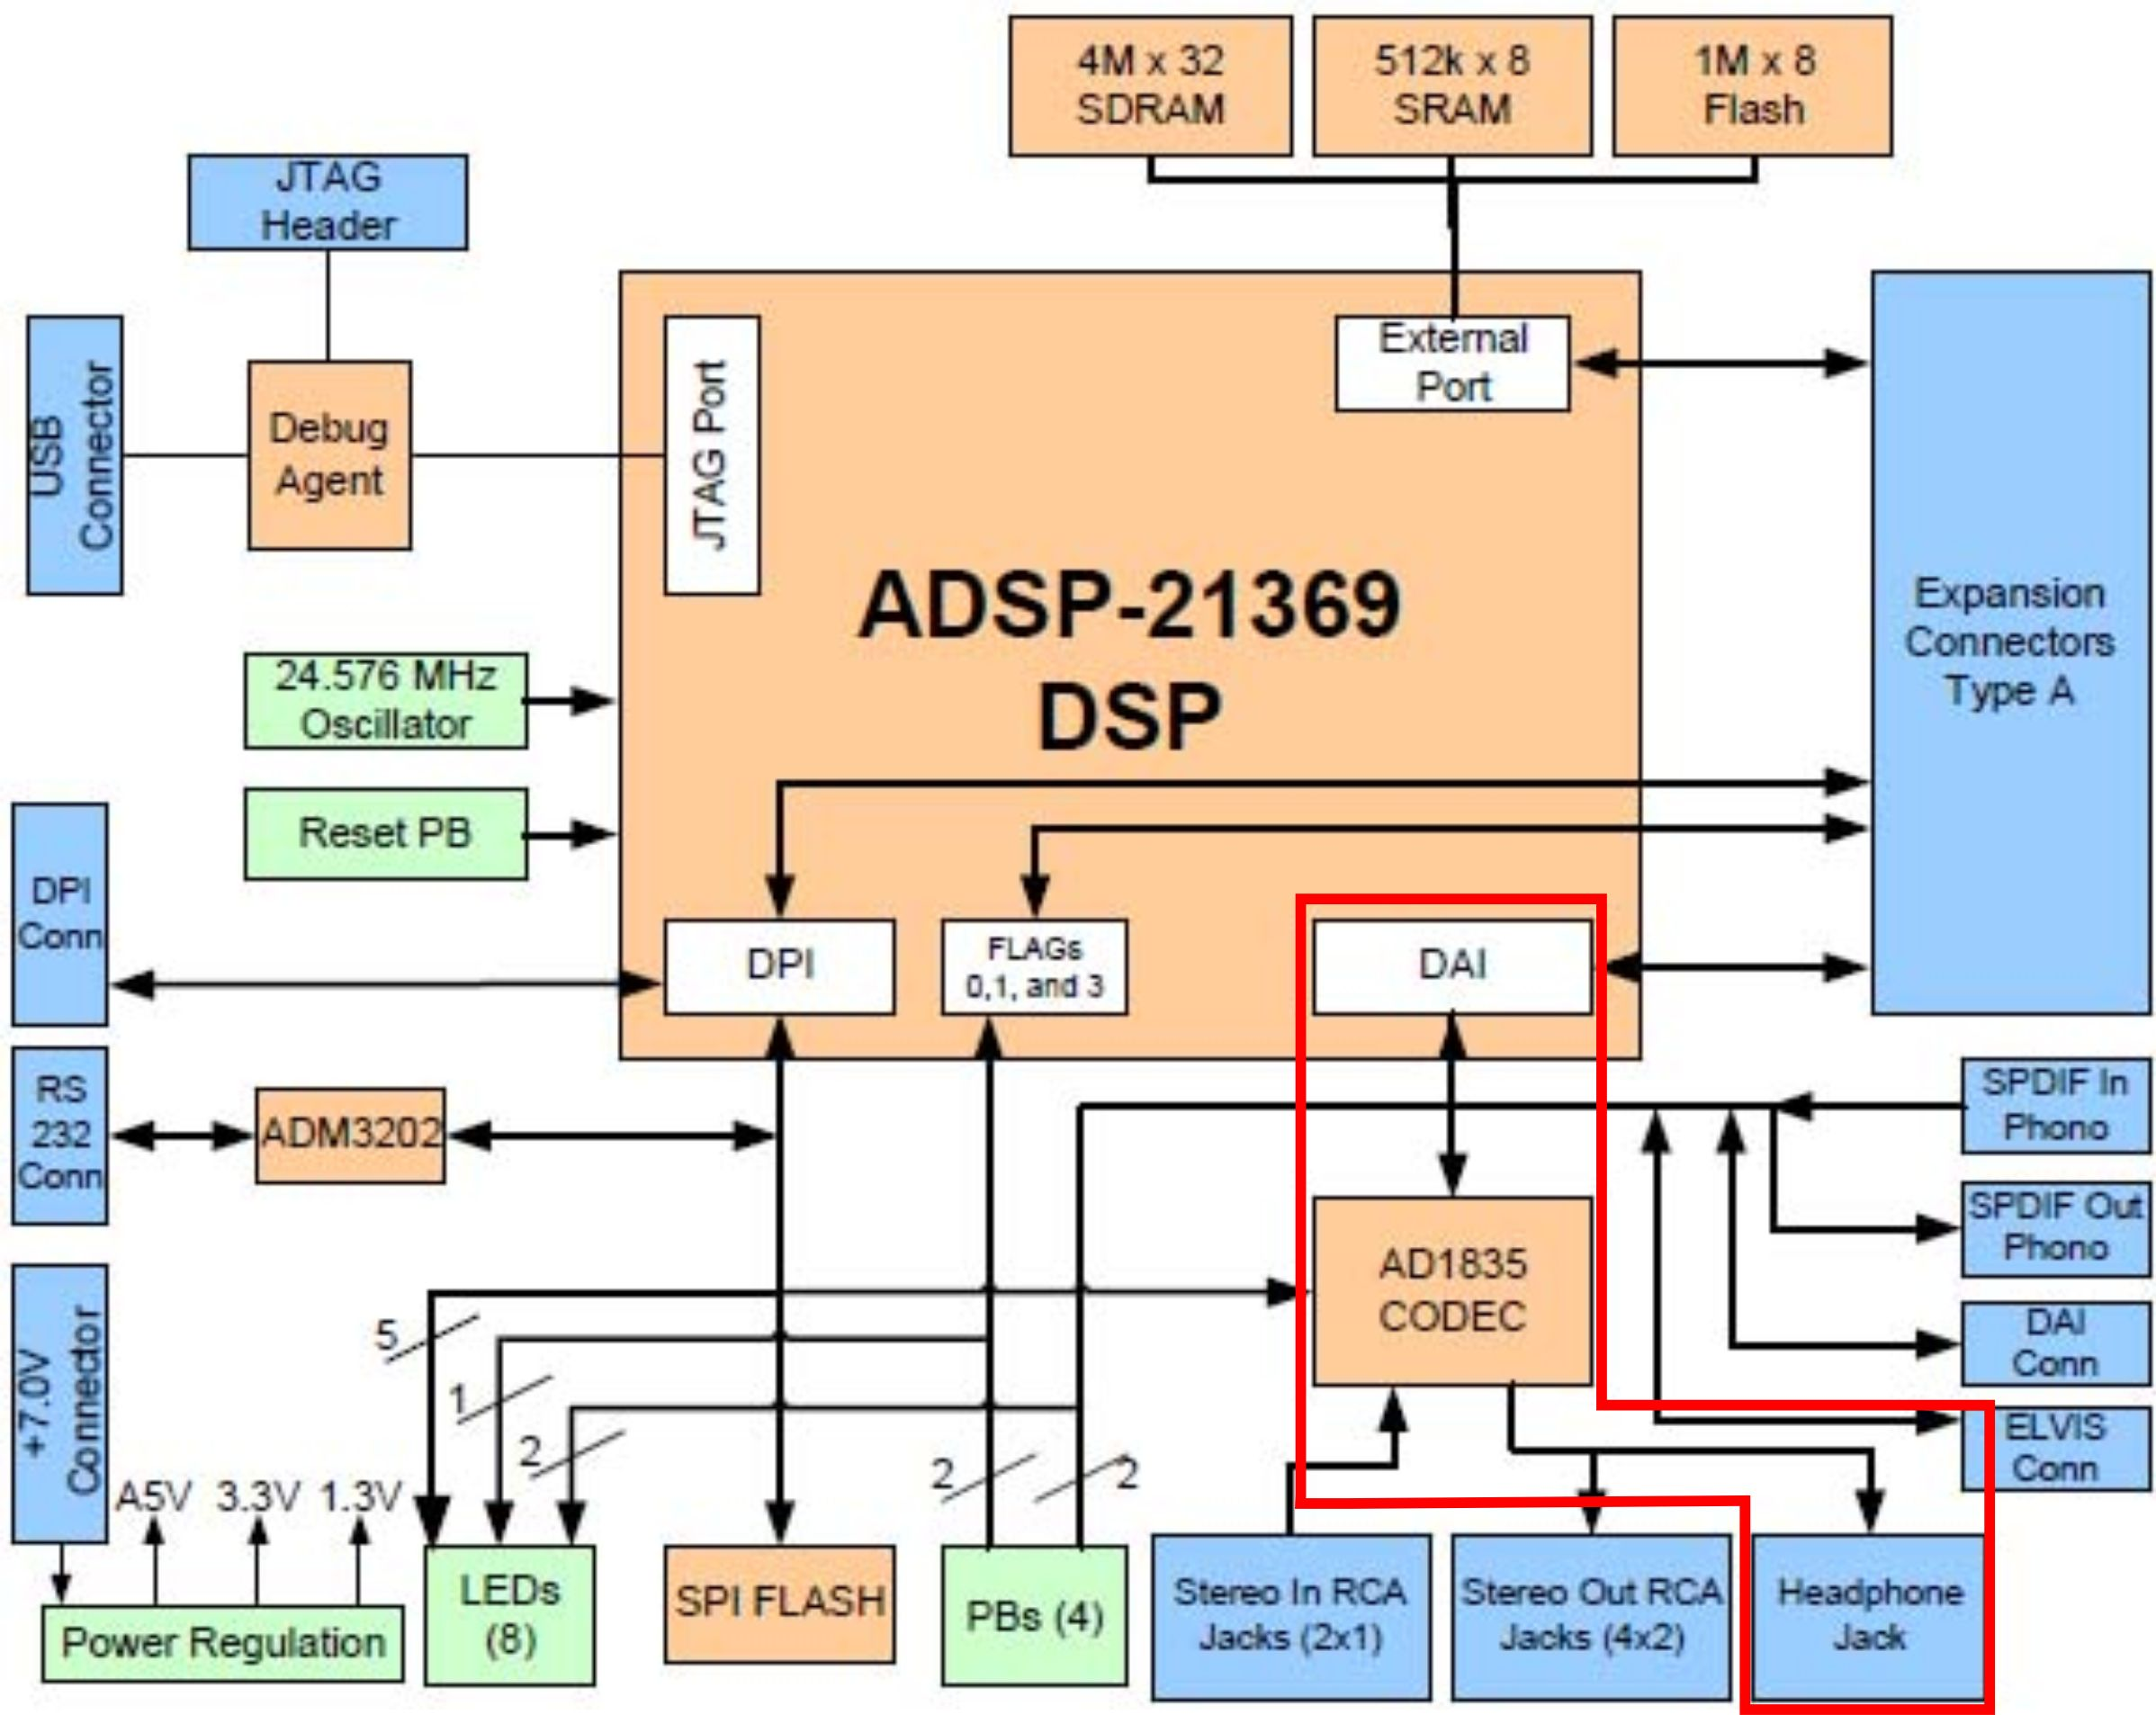
\includegraphics[height=10cm]{systemArchitectureDAI}
\rule{30em}{0.5pt}
\caption{System Architecture Block Diagram}
\label{fig:DAI1}
\end{figure}
\begin{figure}[htbp]
\centering
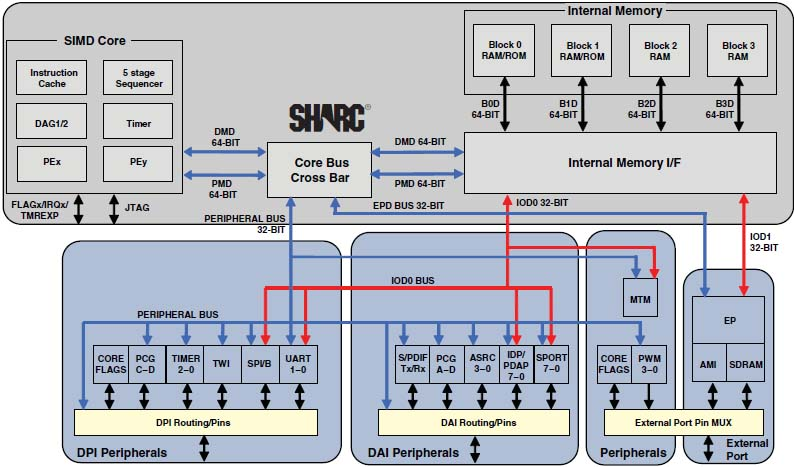
\includegraphics[height=8.4cm]{systemFunctionalDAI}
\rule{30em}{0.5pt}
\caption{Peripherals Architecture Block Diagram}
\label{fig:DAI2}
\end{figure}
%----------------------------------------------------------------------------------------
\subsubsection{Signal Routing Unit (SRC)}
Like is said above, the SRUs are used to connect inputs and outputs. The signals routed by the SRUs are diveded into functional groups. Each group routes a set of signals with a specific purpose. For example, SRU1 Group B routes serial data signals.  It are both the peripherals control registers and the SRU configuration that determine the direction of the signal flow in a pin buffer. \\ To configure the SRU we must thus write values that correspond to signal sources into the bit fields that further correspond to the signal inputs. However the registers are arranged into functional groups, this is stays a very difficult task. In order to ease this coding process one of the following two procedures can be used:
\begin{description}
\item[Expert DAI plug-in:] This software plug-in is included in the VisualDSP++ IDE and greatly simplifies the task of connecting the signals in the SRUs.
\item[sru.h:] This is a macro implementation that automates most of the work of signal assignments and functions. The macro can be used like is shown below to connect the ADC to SPORT0 using data input A. (See file \emph{initSRU.c})
\begin{alltt}
#include <sru.h>;
/* The following lines illustrate how the macro is used: */
/* Route SPORT 1 clock output to pin buffer 5 input */
\hspace{1cm}	SRU(DAI_PB05_O,SPORT0_DA_I);
\end{alltt}
\end{description}
To explain the input/output mnemonic, which always ends with \verb+_I+ if the signal is an input and with \verb+_O+ if the signal is output, we must explain one more thing in this section. Because of the context of the SRU, a pin is not just a pin anymore. Pins are now replaced by logical interfaces (pin buffers), shown in figure \ref{fig:pinbuffer}.
\begin{figure}[htbp]
\centering
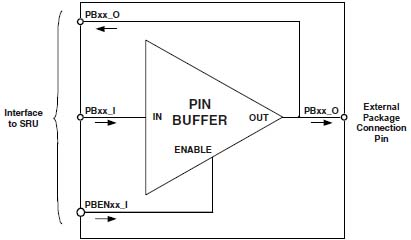
\includegraphics[height=4cm]{pinbuffer}
\rule{30em}{0.5pt}
\caption{Pin Buffer}
\label{fig:pinbuffer}
\end{figure}\\
The interface's input must be thought of as the input to a buffer amplifier which can drive a load on the external pin. The pin buffer enable pin is an input signal that enables the buffer if its value is logic high and disables the buffer when its logic low. When the pin enable is set the output pin is logically equal to pin input. If not, the output of the buffer becomes high impedance and an external device can sent a logic value to the input of the ADSP-21369. The SRU receives this pin as an pin interface output and routes it as an input to the SHARC processor. If pin enable is asserted pin output is equal to pin input (the amplifier then acts as a current source, low impedance). See appendix \ref{AppendixD} for more explanation.
%----------------------------------------------------------------------------------------
\subsubsection{AD1835A}
The pins of the DAI are connected to an AD1835A audio codec. This is a high performance, single-chip codec with four stereo DACs and one stereo ADC, so 8 DACs and two ADCs. \\ The engine has a programmable interpolator which allows the user to select different interpolation rates. By this way the desired sample rate can be selected. For the DACs the user can choose between 48kHz, 96kHz and one DAC even supports 192kHz, see the table below extracted from the AD1835A's datasheet. The location of this chip on the ADSP-21369 is shown in figure \ref{fig:dac1}. Table \ref{tab:dac1} shows the connections between the processors DAI and the AD1835A audio chip. We used the 96kHz sample frequency.\\
\begin{table}[!hb]
\begin{center}
\begin{tabular}[!hb]{|c|c|c|}
\hline
\textbf{Sample Rate} & \textbf{Interpolator Rate} & \textbf{DAC Control 1 Register}\\
\hline
48 kHz & 8x & 000000xxxxxxxx00\\
\hline
96 kHz & 4x & 000000xxxxxxxx01 \\
\hline
192 kHz & 2x & 000000xxxxxxxx10 \\
\hline
\end{tabular}
\caption{AD1835A DAC Sample rate settings}
\label{tab:dac1}
\end{center}
\end{table}
\begin{figure}[htbp]
\centering
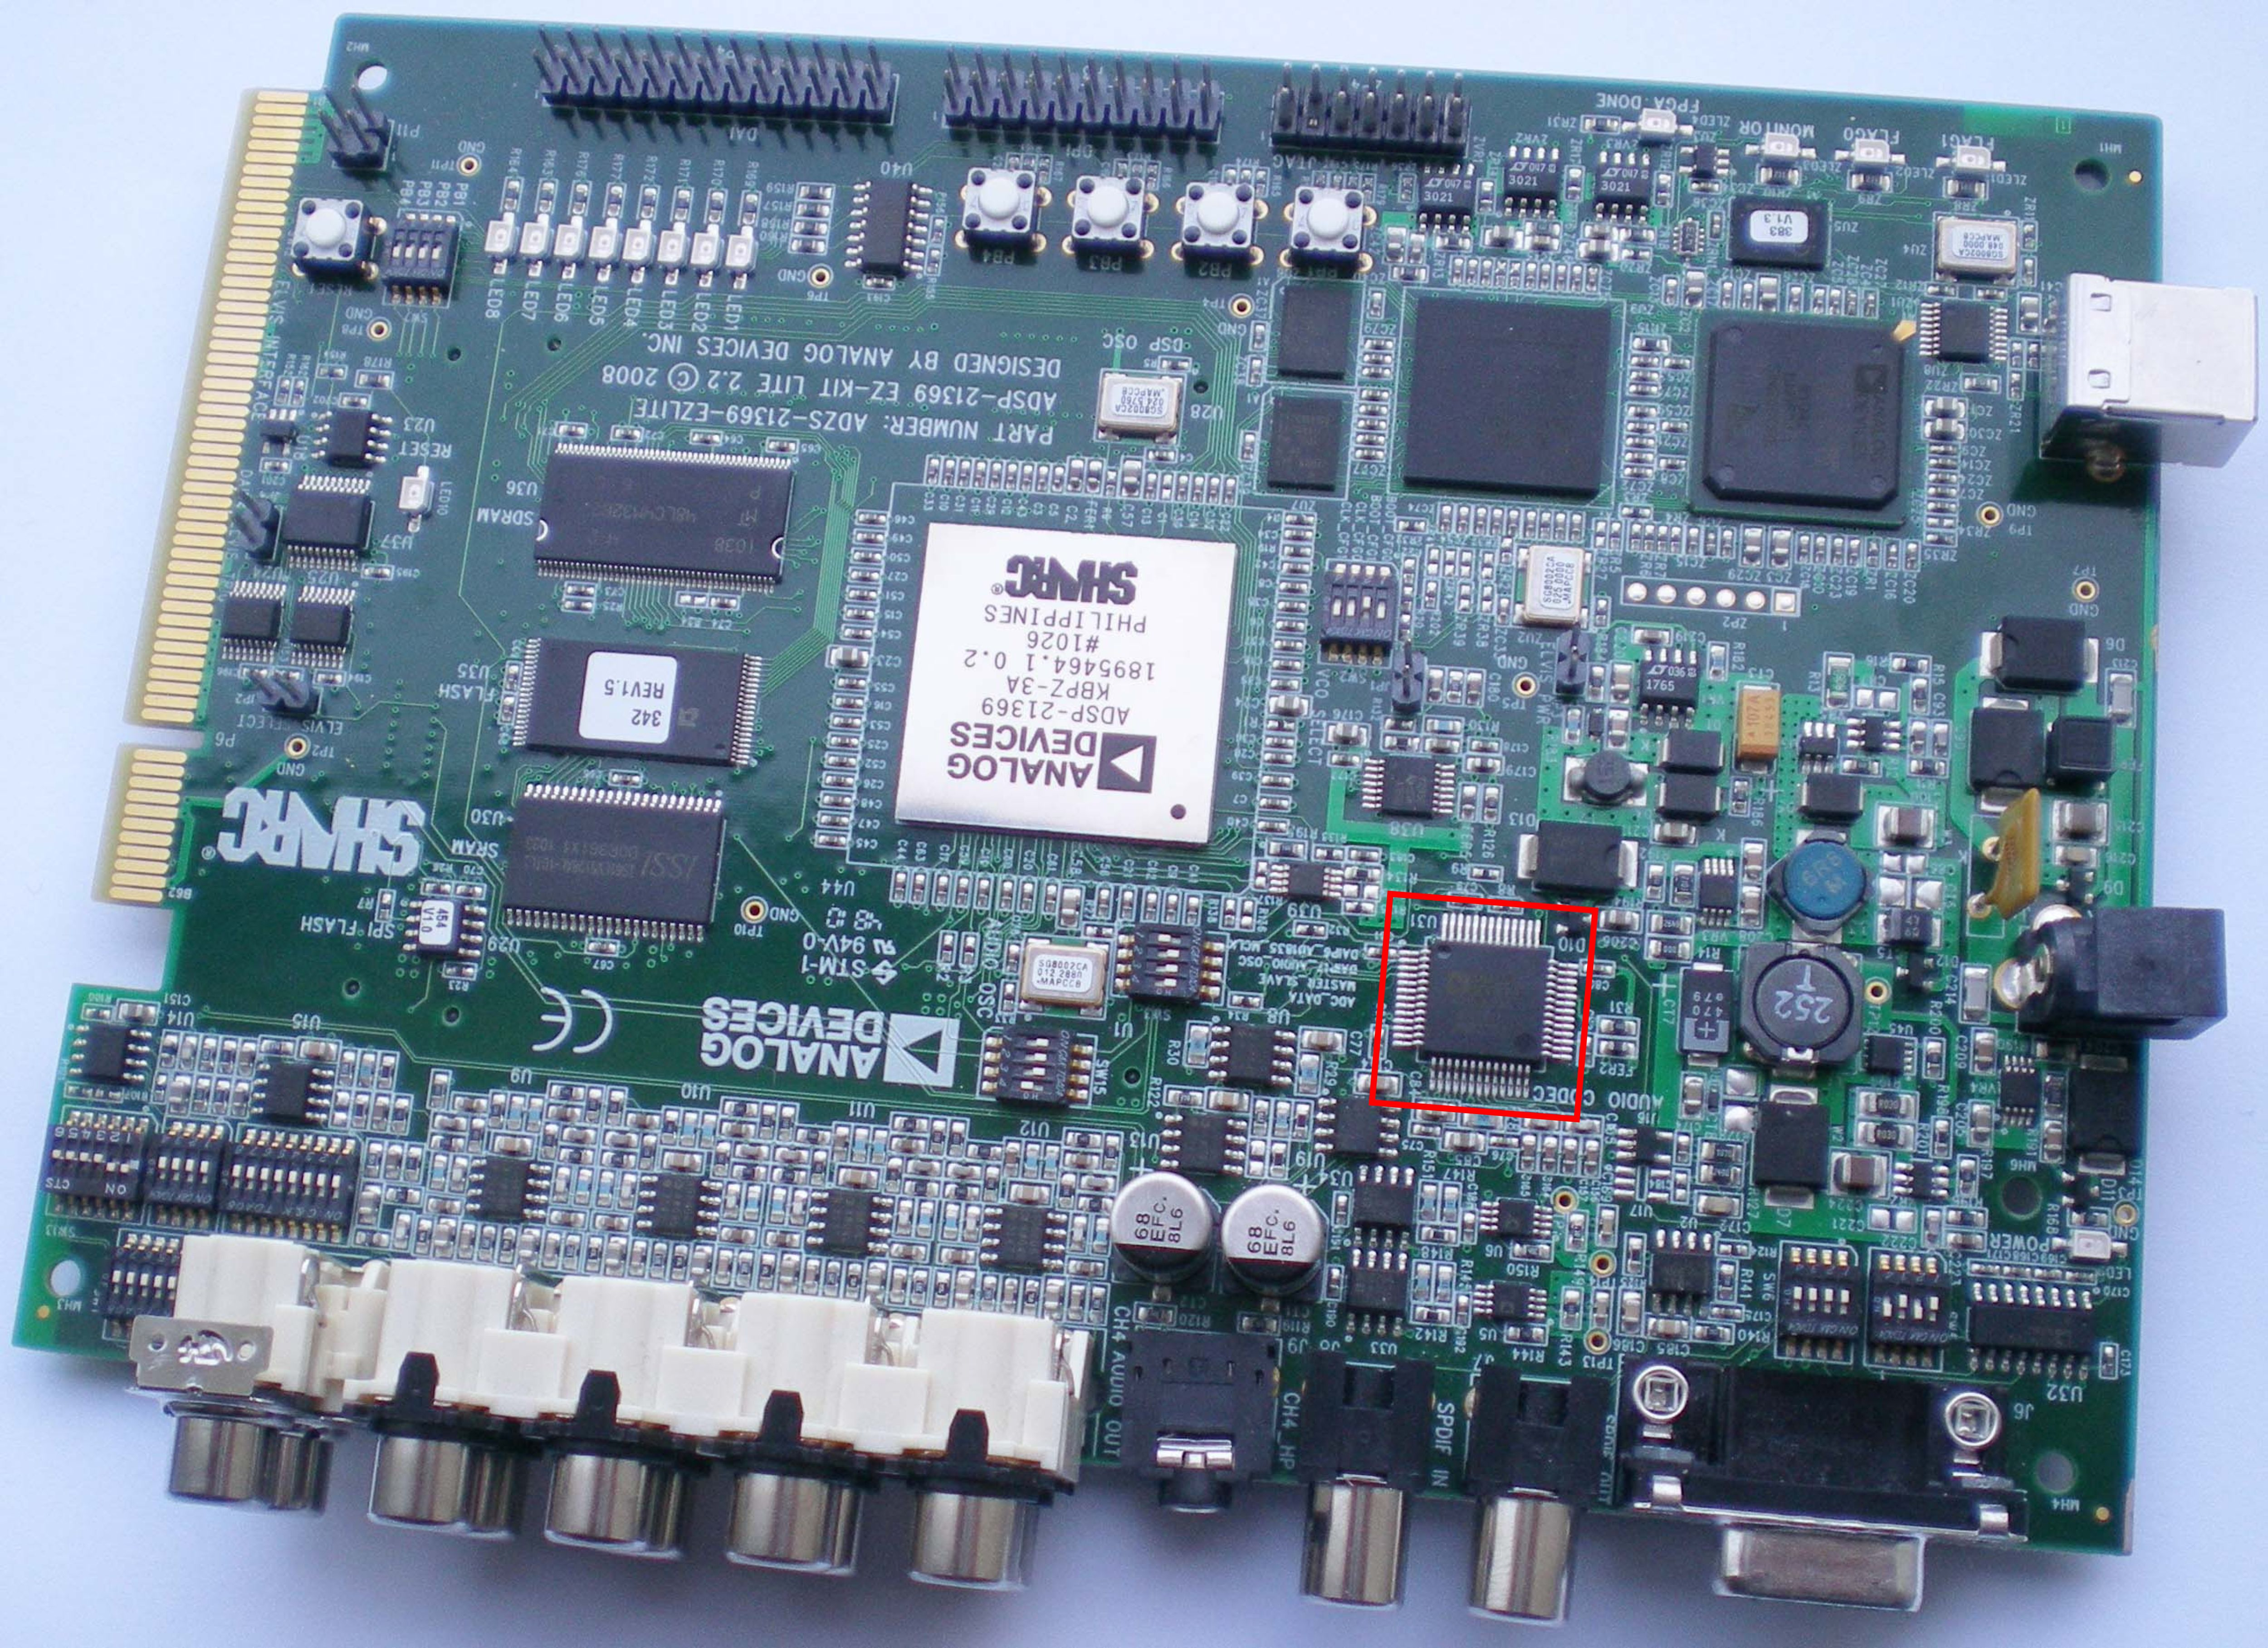
\includegraphics[height=10.5cm]{ad1835A}
\rule{30em}{0.5pt}
\caption{AD1835A on the ADSP-21369 DSP Board}
\label{fig:dac1}
\end{figure}
\begin{figure}[htbp]
\centering
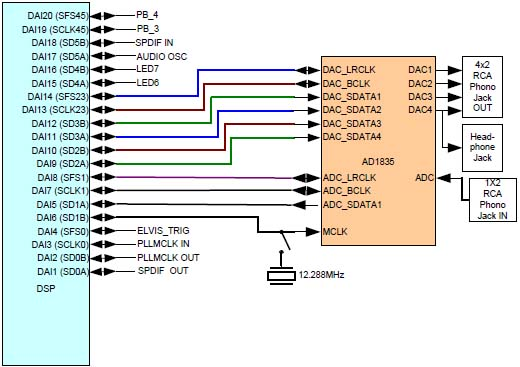
\includegraphics[height=10cm]{ADIAD1835}
\rule{30em}{0.5pt}
\caption{Peripherals Architecture Block Diagram}
\label{fig:ADIAD1835}
\end{figure}\\
To make the AD1835A's four serial data output connections shown in figure \ref{fig:ADIAD1835} we use the macro defined in \emph{$<$sru.h$>$}, which is shown below. For the complete initialization (clock and frame sync) we refer to the file \emph{initSRU.c}.
\begin{alltt}
    SRU(SPORT2_DB_O,DAI_PB09_I);  <-- notice that DAC4 is connected to SPORT2B
    SRU(SPORT2_DA_O,DAI_PB10_I);
    SRU(SPORT1_DB_O,DAI_PB11_I);
    SRU(SPORT1_DA_O,DAI_PB12_I);
\end{alltt}
%----------------------------------------------------------------------------------------
\subsubsection{SPORT}
The previous sections explained how to set up the connections between the DAI and the DAC but we still have to initialize the communication protocol to be used. The ADSP-21369 has eight independent, synchronous serial ports (SPORT) that provide us with an I/O interface. Each SPORT has a set of control registers and data buffers which allows a variety of serial communication protocols.\\ 
\textbf{In the synthesizer program we wil use SPORT2B to communicate from processor to DAC4 in $\mathrm{I^{2}C}$ mode.} The serial data will be transferred automatically from on-chip memory using DMA block transfers in a chained DMA process.
\begin{description}
\item[Chained DMA:] In such a process the block to transfer comes from the (next) chain pointer register. When the current DMA transfer is complete the processor automatically begins the next DMA transfer indicated by the pointer register. To set up a chain of DMA operations the following steps are used:
\begin{enumerate}
\item Set up all TCBs in internal memory: 
\begin{alltt}
	unsigned int Block_A[NUM_SAMPLES] ;
	unsigned int Block_B[NUM_SAMPLES] ;
	unsigned int Block_C[NUM_SAMPLES] ;

	TCB_Block_A[0] = (int) TCB_Block_C + 3 - OFFSET + PCI ;
	TCB_Block_A[3] = (unsigned int) Block_A - OFFSET ;

	TCB_Block_B[0] = (int) TCB_Block_A + 3 - OFFSET + PCI ;
	TCB_Block_B[3] = (unsigned int) Block_B - OFFSET ;

	TCB_Block_C[0] = (int) TCB_Block_B + 3 - OFFSET + PCI ;
	TCB_Block_C[3] = (unsigned int) Block_C - OFFSET ;
\end{alltt}
\item Set up the appropriate DMA control registers: set DMA enable bit \verb+SDEN_B+, set chaining enable bit \verb+SCHEN_B+. This information is written in the $\mathrm{I^{2}C}$ mode control bits of the SPORT, \verb|SPCTLx|. 
\begin{alltt}
	/* Channel enable: SPEN_B
	 * Word length: SLEN24
	 * Operation mode enabled: OPMODE
	 * Activate TXSPxy data buffers and transmit shift registers: SPTRAN
	 */ 
    *pSPCTL2 |= (SPTRAN | OPMODE | SLEN24 | SPEN_B | SCHEN_B | SDEN_B) ;
\end{alltt}
\item Write the adres of the first (next) TCB to the chain pointer register. For our program we use the SPORT Chain Pointer Registers \verb+CPSPx+, so for SPORT2B this gives:
\begin{alltt}
    *pCPSP2B = (unsigned int) TCB_Block_C - OFFSET + 3 ;
\end{alltt}
\end{enumerate}
\end{description}
For the complete initialization of the SPORT please have a look at file \emph{initSPORT.c}. Remark that the data for the transmit buffers \verb+TXSPxA/B+ is loaded automatically by the DMA controller.\\

\begin{description}
\item[SPORT interrupt:] The SPORT DMA mode provides a mechanism to transmit an entire block of serial data and creates an interrupt afterwards rather than after each transmitted word, significantly reducing overhead. \\
As is explained in section \ref{sec:a} all processing of the algorithms must be done before the next block of data is provided. To keep track of this real-time constraint the semaphores \emph{isProcessing} and \emph{blockReady} are introduced and update the real-time flag each time a SPORT DMA interrupt occurs. If the program becomes too slow, real-time is set false and a warning sound will be produced. If the processing is done before the interrupt occurs the SPORT chain pointer register is updated:
\begin{alltt}
	void TalkThroughISR()
	\{
		    if(isProcessing) //still busy calculating
		    realtime=0;
    
		    (int_cntr++);		//Increment the block pointer
		    int_cntr %= 3;
	
		    blockReady = 1;
	\}
\end{alltt}
\end{description}
%----------------------------------------------------------------------------------------
\section{The DSP Synthesizer program}
All instructions for the Sharc processor are written in C or assembly. Once finished all source code is translated and linked by the compiler integrated in VisualDSP++. Then this executable machine code is uploaded to the device.
\subsection{Program execution}
To follow the next descriptions please take a look at figure \ref{fig:flowChart}. The \emph{main.c} file contains the central starting point, namely the \verb+main()+ function. At run time, the execution will start at the first line of this function. In our case this is a series of \verb+Init()+ functions, which were briefly discussed in the previous section.\\
Once all initializations are done the real work can be started. At this point we enter the \verb+while(!stop)+ loop. As long as the user does not press the stop button the microprocessor continues running and must do something, so an infinite loop keeps it busy. This is typically for embedded controllers.\\ Next is another while loop: \verb+while(blockReady)+. After the previous block has been processed and the SPORT DMA interrupt has occured the next block can be processed. This next block will either produce the pursuit of the previous frame or will produce a warning tone, indicating that the calculations on the previous block were not finished before the block was needed by the DAC, and thus the signal could not be produced in realtime. We will first explain the not-realtime case since this will also be helpful in the realtime process.
\begin{figure}[htbp]
\centering
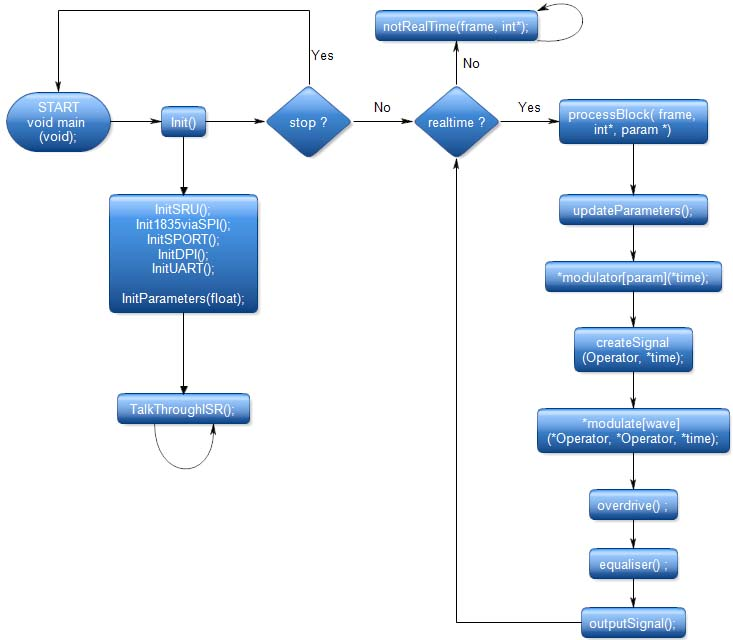
\includegraphics[height=13cm]{flowChart}
\rule{30em}{0.5pt}
\caption[Flow chart of the DSP Synthesizer program]{Flow chart of the DSP Synthesizer program\\(Compare this figure with figure \ref{fig:funDesign} ) }
\label{fig:flowChart}
\end{figure}\\
\subsubsection{Not-realtime} \label{secb}
The not-realtime-function takes two parameters as argument, both pointers and creates a 8000Hz warning tone. The first pointer is the address of the array containing the samples to be processed. This array contains 1024 samples and is contained in a TCB block, used by the DMA chain to feed the DAC. The second is a simple int pointer which is used to indicate which particular samples to create, fulfilling the role as the time of the sine function in this case.\\ 
\begin{alltt}
void notrealtime(unsigned int *block_ptr, int *time)
\{
	   int i;
	   float scalar = powf(2.0,23.0); 
	   long j,N,readptr,ref;

	   //Clear the Block Ready Semaphore, Set the isProcessing Semaphore before starting
	   blockReady = 0;
	   isProcessing = 1;

	   for(i=0;i<NUM_SAMPLES;i++)
	   \{
      	*(block_ptr+i) = 0.1*scalar*sin(2.0*3.141592*8000.0/sampleFreq * ( (int)(*time)++ ));
      	(*time)%=sampleFreq;	
	   \}

    //Clear the Processing Active Semaphore after processing is complete
    isProcessing = 0;
\}
\end{alltt}
%----------------------------------------------------------------------------------------
\subsubsection{Realtime: let's play}
In order to easily manipulate our sound processing algorithms we need the same arguments as indicated in section \ref{secb} plus an addiditonal pointer used to communicate with the Labview interface.
\begin{description}
\item[Refresh parameters:] Before we start to create our signal we first fetch the parameters as the user defines them in the Labview interface. Those values are put into global variables so they have a reserved spot in the program memory.
\item[Select modulation type:] Depending on which modulation algorithm the user selects a different function will be executed. This is almost literally the definition of function pointers, isn't it? Since the different modulation modes have a fixed value in the labview interface we can define the function pointers very efficiently. The definition of the function pointer we used is a function that takes one int pointer as argument end returns void. Below the creation and call of the (fancy) function pointers is shown:
\begin{alltt}
	Modulation *modulator[4] = \{&TwoOperators, &ThreeOperators, &FourOperators, 
								&FourOperatorsPlus\};

	(*modulator[(int) parameters[0]])(time);
\end{alltt}
\item[Create and modulate signal:] For efficiency reasons we mostly pass arguments by reference. However in the case below we use pass by value because we don't want to adapt the value of the pointer immediately (and copying the value to a local variable is also a bit sloppy). So to create and modulate the signal first dereference the time pointer received by the function pointer:
\begin{alltt}
	void TwoOperators(int *t)
	\{
	   int i;
	   Operator *carrier = &op[0];
	   Operator *modulator = &op[1];
	
	   createSignal(modulator, *t);		
	   (*modulate[carrier->wave])(carrier, modulator, *t);
	\}
\end{alltt}
As you can see, the modulation algorithm also depends on which type of wave is selected and this is also fixed with function pointers. For the complete implementation of the modulate algorithms we refer to the file \emph{operator.c}.
\item[Overdrive:] If the effect is enabled the function overdrive is called. This function takes as arguments operator 0 and a pointer to the effect's parameters. The creation and modulation algorithms are so that operator 0 always contains the whished signal, this is why it is used as argument here and in the next functions.
\begin{alltt}
	if( effect.enabled ) overdrive(&op[0], &effect);
\end{alltt}
\item[Equaliser:] If the equaliser is enabled the following function is called: 
\begin{alltt}
	if( equaliser.enabled ) enableEqualiser(&op[0], &equaliser);
\end{alltt}
\item[Output signal:] Now we have fully modulated our signal we still have to put it into the TCBs to send it to DAC4. One last thing that is added here is a control of the overal gain of the signal. \\ We may not forget that because we wanted to use the timing values several times we used a pass by value. That's why after the whole frame is processed we still have to update the time reference.
\begin{alltt}
	for(i=0;i<NUM\_SAMPLES;i++)
	\{	
       *(block\_ptr+i) = (unsigned int)(signed int)(op[0].signal[i] * 
       								    	  Gain(\&equaliser)*0.1*scalar );
	\}
	(*time)+= 1024;  
	(*time)%=sampleFreq;
\end{alltt}
\end{description}
%----------------------------------------------------------------------------------------
\subsection{Key functions}
\begin{description}
\item[void createSignal(Operator *, int)] \label{code:createSignal}
\begin{alltt}
\{
	   int i;
	   switch(op->wave)
	   \{	
	   case SINE:
		      for(i=0; i<NUM_SAMPLES; i++)
		      \{
	            op->signal[i] = envelope(op) * sin( 2.0 * 3.141592 * 
	      		   				          op->frequency / sampleFreq * t++ );
		      \}
		      break;
	   case TRIANGULAR:
		      for(i=0; i<NUM_SAMPLES; i++)
		      \{
	            op->signal[i] = 1-(fabs((t++*op->frequency%sampleFreq)-sampleFreq/2)
	                         / (sampleFreq/4)  - 1 );
	            op->signal[i] *= envelope(op);
		      \}
		      break;
	   case SAWTOOTH:
		      for(i=0; i<NUM_SAMPLES; i++)
		      \{
	            op->signal[i] = 2*( t++*(op->frequency)%sampleFreq )/sampleFreq - 1;
	            op->signal[i] *= envelope(op);
		      \}
		      break;		
	   default:
		      break;
	   \}		
\}

\end{alltt}

\textbf{\textcolor{red}{Remark:} Why is there no t\%=sampleFreq in this function?} \\ 
\item[void ModulateSine(Operator *carrier, Operator *modulator, int t)] Please remember formula \ref{eq:fmb} discussed in chapter 2 on frequency modulation. 
\begin{alltt}
   int i;
   for(i=0; i<NUM_SAMPLES; i++)
   \{
      carrier->signal[i] = sin( 2.0 * 3.141592 * carrier->frequency / 
             						     sampleFreq * t++ + (modulator->signal[i]) );
      carrier->signal[i] *= envelope(carrier);
   \}
\end{alltt}
\end{description}
